\documentclass[10pt]{article}
\usepackage[a4paper,margin=5mm,landscape]{geometry}
\usepackage{blindtext}

\usepackage{multicol}
\usepackage{enumitem}
\usepackage[dvipsnames]{xcolor}
\usepackage{graphicx}



\usepackage[condensed,math]{iwona}

\usepackage[sfdefault,condensed]{roboto}  %% Option 'sfdefault' only if the base font of the document is to be sans serif
\usepackage[T1]{fontenc}


% Marca d'agua
%\usepackage{draftwatermark}
%\SetWatermarkText{Draft}
%\SetWatermarkScale{5}

\setlength{\columnseprule}{.5pt}
\linespread{.95}

\usepackage{titlesec}
\titlespacing{\subsection}{0pc}{3.pt}{1.pt}
\titlespacing{\subsubsection}{0pc}{1.5pt}{1.pt}

\definecolor{mygray}{RGB}{250, 250, 250}
\pagecolor{mygray}

\usepackage{float}

\setlength{\textfloatsep}{1pt}
\setlength{\floatsep}{1pt}
\setlength{\intextsep}{1pt}

\begin{document}
\noindent
{\Large{\textbf{\emph{C++ Standard Template Library (STL) Quick Reference}}, {\small version 1.0}}	
}

\noindent
{\small  Roberto D. Algarte (2024)}

\scriptsize
\begin{multicols*}{5}
{\color{Blue}
\subsection*{CONTAINERS}	
\noindent
Aggregates of elements that provide element insertion, removal and access.

\subsubsection*{\textsc{Theory} - \emph{Time Complexity}} 
\begin{figure}[H]
\begin{center}
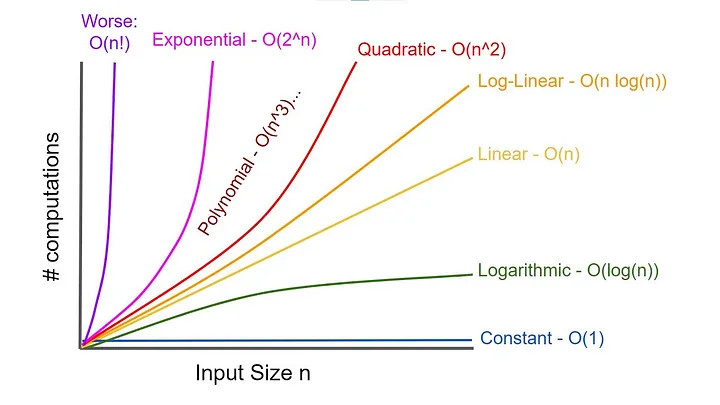
\includegraphics[scale=.21]{complexity.jpg}	
\end{center}
\end{figure}

\subsubsection*{\textsc{Theory} - \emph{Linear Aggregates}} 

\begin{itemize}[leftmargin=*,topsep=0.25pt]
  \setlength\itemsep{.3pt}
	\item \emph{Array}: static or dynamic structure whose elements have defined positions and are stored in contiguous memory. Insertion and removal of elements may imply repositioning of other elements or repositioning of the entire structure; 
	\item \emph{Linked list}: dynamic structure whose elements may not be stored contiguously. A node (list element) is composed by a value and one or two references to adjacent nodes. Nodes of a \emph{doubly-linked} list have two references, and of a \emph{singly-linked}, one reference. Insertion and removal don't imply repositioning of other elements;
	\item \emph{Stack}: LIFO dynamic structure with one end, in which insertion, deletion and access are performed;
	\item \emph{Queue}: FIFO dynamic structure with two ends, one for insertion and another for removal; access can be performed on both. In a \emph{double-ended} queue, both ends allow insertion and removal;  
\end{itemize}

\subsubsection*{\textsc{Sequence Containers}} 
\noindent
Containers whose elements can be accessed sequentially and are stored contiguously in memory.

\begin{itemize}[leftmargin=*,topsep=0.25pt]
  \setlength\itemsep{.3pt}
	\item \textbf{array} @ $<$array$>$: wrapper for C static arrays;
	\item \textbf{vector} @ $<$vector$>$: implementation of a dynamic array. Insertion and removal are $O(1)$ at the end, $O(n)$ elsewhere; access is $O(1)$;
	\item \textbf{dequeue} @ $<$dequeue$>$: implementation of a double-ended queue. Insertion, removal and access are $O(1)$;
	\item \textbf{forward\_list} @ $<$forward\_list$>$: implementation of a singly-linked list. Insertion and removal are $O(1)$; access is $O(n)$. Provided by $<$forward\_list$>$;  
	\item \textbf{list} @ $<$list$>$: implementation of a doubly-linked list. Insertion and removal are $O(1)$; access is $O(n)$;
\end{itemize}

\subsubsection*{\textsc{Sequence Container Adapters}} 
\noindent
Wrappers created around dequeue to provide other types of aggregates.

\begin{itemize}[leftmargin=*,topsep=0.25pt]
  \setlength\itemsep{.3pt}
	\item \textbf{stack} @ $<$stack$>$: implementation of a stack;
	\item \textbf{queue} @ $<$queue$>$: implementation of a simple queue;
	\item \textbf{priority\_queue} @ $<$queue$>$: implementation of a queue in which the front element must observe a priority condition (the largest, by default). Insertion and removal are $O(log(n))$;
\end{itemize}
\noindent

\subsubsection*{\textsc{Associative Containers}} 
\noindent
Containers constituted by (non)primary key sorted elements or pair of (non)primary key-value sorted elements that are  inserted, removed and accessed in $O(log(n))$ time complexity for the worst case.

\begin{itemize}[leftmargin=*,topsep=0.25pt]
  \setlength\itemsep{.3pt}
	\item \textbf{set} @ $<$set$>$: constituted by primary key elements;
	\item \textbf{map} @ $<$map$>$: constituted by primary key-value elements;
	\item \textbf{multiset} @ $<$set$>$: constituted by non primary key elements;
	\item \textbf{multimap} @ $<$map$>$: constituted by non primary key-value elements;  
\end{itemize}
\noindent
Each one of these types has its \textbf{unordered\_*} counterpart, whose elements are inserted or removed in $O(1)$, and accessed in $O(n)$ for the worst case. 


}

\par\noindent\rule{155pt}{0.4pt}

{\color{Blue}
\subsection*{I/O STREAMS}	
\noindent
Streams enable flow of data to be written (output) or to be read (input). Output streams can be buffered or not.
The \emph{extractor operator} $<<$ when applied to input streams performs formatted input while the \emph{insertion operator} $>>$ applied to output streams performs formatted output. 

\subsubsection*{\textsc{Console Streams}} 
\begin{itemize}[leftmargin=*,topsep=0.25pt]
  \setlength\itemsep{.3pt}
	\item \textbf{cin} @ $<$iostream$>$: wrapper around the standard C stream stdin, which reads data from the console;
	\item \textbf{cout} @ $<$iostream$>$: wrapper around the standard C stream stdout, which writes data to the console and is buffered;
	\item \textbf{cerr} @ $<$iostream$>$: wrapper around the standard C stream stderr, which writes data to the console;
\end{itemize}

\subsubsection*{\textsc{String Streams}}
\noindent
Streams that enable flow of outputted or inputted strings.

\begin{itemize}[leftmargin=*,topsep=0.25pt]
  \setlength\itemsep{.3pt}
	\item \textbf{basic\_istringstream} @ $<$sstream$>$: provides high level string input formatting;
	\item \textbf{basic\_ostringstream} @ $<$sstream$>$: provides high level string output formatting;
	\item \textbf{basic\_stringstream} @ $<$sstream$>$: provides high level string input/output formatting;
\end{itemize}


\subsubsection*{\textsc{File Streams}} 
\noindent
Streams that enable flow of outputted or inputted data to or from files.

\begin{itemize}[leftmargin=*,topsep=0.25pt]
  \setlength\itemsep{.3pt}
	\item \textbf{basic\_ifstream} @ $<$fstream$>$: provides high level file input formatting;
	\item \textbf{basic\_ofstream} @ $<$fstream$>$: provides high level file output formatting;
	\item \textbf{basic\_fstream} @ $<$fstream$>$: provides high level file input/output formatting;
\end{itemize}

\subsubsection*{\textsc{Aliases}} 
\begin{itemize}[leftmargin=*,topsep=0.25pt]
  \setlength\itemsep{.3pt}
	\item \textbf{istringstream} $=$ \textbf{basic\_istringstream}<char>;
	\item \textbf{ostringstream} $=$ \textbf{basic\_ostringstream}<char>;
	\item \textbf{stringstream} $=$ \textbf{basic\_stringstream}<char>;
	\item \textbf{ifstream} $=$ \textbf{basic\_ifstream}<char>;
	\item \textbf{ofstream} $=$ \textbf{basic\_ofstream}<char>;
	\item \textbf{fstream} $=$ \textbf{basic\_fstream}<char>;
\end{itemize}


}

\par\noindent\rule{155pt}{0.4pt}

{\color{Blue}
\subsection*{ITERATORS}	
\noindent
Pointer-like types created to implement the iterator pattern in STL. The iterator pattern states that aggregate structures and element-accessing functions should be decoupled.

\subsubsection*{\textsc{Iteratable Aggregates}} 
\noindent
All types of STL containers, C arrays, input and output streams.

\subsubsection*{\textsc{Concepts}} 
\begin{itemize}[leftmargin=*,topsep=0.25pt]
  \setlength\itemsep{.3pt}
	\item \textbf{output\_iterator} @ $<$iterator$>$: a type that can be both pre- and post-incremented, related to a given structure to which values can be written (e.g. output streams);
	\item \textbf{ostream\_iterator} @ $<$iterator$>$: a specific type of out\-put\_i\-te\-ra\-tor that writes to an output stream;
	\item \textbf{input\_iterator} @ $<$iterator$>$: a type that can be both pre- and post-incremented, related to a given structures whose values can be read (e.g. input streams);
	\item \textbf{istream\_iterator} @ $<$iterator$>$: a specific type of in\-put\_i\-te\-ra\-tor that reads from an input stream;
	\item \textbf{forward\_iterator} @ $<$iterator$>$: an input\_iterator that has equality comparison and multi-pass, which means that it can traverse multiple times the elements of an aggregate (e.g. containers); 
	\item \textbf{bidirectional\_iterator} @ $<$iterator$>$: a forward\_iterator able to traverse backwards; 
	\item \textbf{random\_access\_iterator} @ $<$iterator$>$: a bidirectional\_iterator that supports subscripting with $O(1)$ time access to elements; 
	\item \textbf{contiguous\_iterator} @ $<$iterator$>$: a specific ran\-dom\_ac\-cess\_i\-te\-ra\-tor that traverses elements stored contiguously in memory (e.g. vector). 
\end{itemize}

\subsubsection*{\textsc{Range Functions}} 
\begin{itemize}[leftmargin=*,topsep=0.25pt]
  \setlength\itemsep{.3pt}
	\item  \emph{\textbf{begin}} @ $<$iterator$>$: returns the first element read-write iterator. The function \emph{\textbf{cbegin}} returns the read-only version;
	\item  \emph{\textbf{end}} @ $<$iterator$>$: returns the one-past-the-last element read-write iterator. The function \emph{\textbf{cend}} returns the read-only version;
	\item  \emph{\textbf{rbegin}} @ $<$iterator$>$: returns the first element read-write reverse iterator. The function \emph{\textbf{crbegin}} returns the read-only version;
	\item  \emph{\textbf{rend}} @ $<$iterator$>$: returns the one-past-the-last element read-write reverse iterator. The function \emph{\textbf{crend}} returns the read-only version;
\end{itemize}

\subsubsection*{\textsc{Adapters}} 
\noindent
Iterator wrappers created to encapsulate some important iterator-related functionalities. 
\begin{itemize}[leftmargin=*,topsep=0.25pt]
  \setlength\itemsep{.3pt}
	\item \textbf{reverse\_iterator} @ $<$iterator$>$: performs reverse order traversal. This adapter can be created by the helper function \emph{\textbf{make\_reverse\_iterator}};
	\item \textbf{move\_iterator} @ $<$iterator$>$: performs move of elements from one aggregate to another. This adapter can be created by the helper function \emph{\textbf{make\_move\_iterator}};
	\item \textbf{insert\_iterator} @ $<$iterator$>$: performs insertion of element at a specified position. This adapter can be created by the helper function \emph{\textbf{inserter}};
	\item \textbf{back\_insert\_iterator} @ $<$iterator$>$: performs back insertion of elements. This adapter can be created by the helper function \emph{\textbf{back\_inserter}};
	\item \textbf{front\_insert\_iterator} @ $<$iterator$>$: performs front insertion of elements. This adapter can be created by the helper function \emph{\textbf{front\_inserter}};
\end{itemize}

\subsubsection*{\textsc{Operations}} 
\begin{itemize}[leftmargin=*,topsep=0.25pt]
  \setlength\itemsep{.3pt}
	\item  \emph{\textbf{distance}} @ $<$iterator$>$: returns the number of elements between two iterators in which the first is included and last excluded;
	\item  \emph{\textbf{advance}} @ $<$iterator$>$: advances an iterator by a given distance;
	\item  \emph{\textbf{next}} @ $<$iterator$>$: increments an iterator and returns it;
	\item  \emph{\textbf{prev}} @ $<$iterator$>$: decrements an iterator and returns it;
\end{itemize}

\par\noindent\rule{155pt}{0.4pt}

{\color{Blue}
\subsection*{ALGORITHMS}	
\blindtext

\subsubsection*{\textsc{Sub 1}} 
\blindtext


\subsubsection*{\textsc{Sub 2}} 
\blindtext


\subsubsection*{\textsc{Sub 3}} 
\blindtext


}

}
\end{multicols*}
\end{document}
